% \begin{savequote}[8cm]
% Alles Gescheite ist schon gedacht worden.\\
% Man muss nur versuchen, es noch einmal zu denken.

% All intelligent thoughts have already been thought;\\
% what is necessary is only to try to think them again.
%   \qauthor{--- Johann Wolfgang von Goethe \cite{von_goethe_wilhelm_1829}}
% \end{savequote}

\chapter{\texorpdfstring{Neutral kaon \CP violation and material\\interaction in BPGGSZ measurements}{Neutral kaon CP violation and material interaction in BPGGSZ measurements}}
\label{ch:4-KS-CPV}

The presence of a \KS meson in the $\D\to\KS h^+h^-$ final states introduces a small bias in BPGGSZ measurements due to \CP-violation in the neutral kaon sector and asymmetries caused by the interaction between the neutral kaons and detector material. These fundamental physics effects are reviewed in Section~\ref{sec:cp_violation_and_material_interaction_of_neutral_kaons}, after which the chapter presents a detailed analysis of the impact on the \lhcb measurement that is the subject of the thesis,  as well as future $\gamma$ measurements with the Belle II experiment. 
Prior to this analysis, the only existing work on the the effect on $\gamma$ measurements suggested a small effect in \BtoDK measurements but potentially \emph{very} significant effects in measurements based on \BtoDpi decays~\cite{grossmanEffectsBarMixing2014}. However, as described in Section~\ref{sub:a_first_look_at_the_impact_on_gamma}, the analysis in Ref.~\cite{grossmanEffectsBarMixing2014} does not take into account the fundamental aspect of the BPGGSZ method: that it relies on the phase-space distribution of signal decays, not phase-space integrated asymmetries. Furthermore, the earlier study only considers the \CP-violation effect, not material interaction. Therefore, a more detailed study was necessary before the \BtoDpi decay mode could reliably be promoted to a signal channel. The full analysis shows the impact on the $\gamma$ measurement in Chapter~\ref{ch:5-GGSZ-measurement} to be small, and allows for the assignment of an appropriate systematic uncertainty.



\section{CP violation and material interaction of neutral kaons} % (fold)
\label{sec:cp_violation_and_material_interaction_of_neutral_kaons}

A brief review of the general phenomenology of mixing and \CP violation in the neutral kaon system is useful, before analysing the impact on $\gamma$ measurements. The presentation in this section follows the PDG review of \emph{\CP violation in the quark section}~\cite{PDG2020}. The general theory considers any pair of neutral mesons $\ket \Mz$ and $\ket \Mzb$ related by \CP conjugation
\begin{subequations}
\begin{align}
     \CP \ket \Mz  &= e^{i\phi_M} \ket \Mzb     &
     \CP \ket \Mzb &= e^{-i\phi_M}\ket \Mz ,
 \end{align} 
 where $\phi_M$ is an arbitrary phase. In this thesis, the convention $\phi_M=0$ is chosen to equal zero, so that
 \begin{align}\label{eq:CP_convention}
     \CP \ket \Mz  &= \ket \Mzb     &
     \CP \ket \Mzb &= \ket \Mz.
 \end{align}
 \end{subequations}
A meson state that starts as a general superposition of $\ket \Mz$ and $\ket \Mzb$ states
\begin{align}
\begin{split}
       \psi_M^0\equiv \psi_M(0) &= a(0)\ket \Mz + b(0)\ket \Mzb \\&\equiv \psi_{\Mz}^0 + \psi_{\Mzb}^0
    \end{split}
\end{align}
will, over time, evolve into a state that consists of a different superposition of $\ket \Mz$ and $\ket \Mzb$, as well as components for all possible states the meson system can decay into
\begin{align}
\begin{split}
     \psi_M(t) &= a(t)\ket \Mz + b(t)\ket \Mzb + \sum c_i(t) f_i \\&\equiv \psi_{\Mz}(t) + \psi_{\Mzb}(t) + \sum c_i(t) f_i.
\end{split}
 \end{align} 
 For time scales that are longer than the typical strong-interaction, the time evolution of the \Mz--\Mzb superposition can be described by a $2\times 2$ Hamiltonian
 \begin{align}
      \frac{\text d}{\text dt} \begin{pmatrix}\psi_{\Mz}(t)\\\psi_{\Mzb}(t)\end{pmatrix} = -i\mathcal H_0 \begin{pmatrix}\psi_{\Mz}(t)\\\psi_{\Mzb}(t)\end{pmatrix}
  \end{align} 
 that is \emph{non-Hermitian} (to allow for decay) but can be parameterised in terms of two Hermitian matrices $\mathcal M$ and $\Gamma_0$
 \begin{align}
     \mathcal H_0 = \mathcal M - \frac{i}{2}\Gamma_0.
 \end{align}
 The quantum states with well-defined (real) masses, $m_j$, and (real) decay widths, $\Gamma_j$, are the two eigenstates of $\mathcal H_0$ with eigenvalues $\lambda_j = m_j - \frac{i}{2}\Gamma_j$. The eigenstates (of course) evolve independently in time, so that
 \begin{align}\label{eq:vac_time_dep}
     \psi_j(t) &= e^{-i\lambda_{j}t} \psi_{j}^0 =  e^{-im_{j}t -\frac{\Gamma_{j}}{2}t}\psi_{j}^0.
 \end{align}
 The eigenstates are denoted $H$ and $L$  according to the size of $m_j$, the real part of the eigenvalues, such that $m_H > m_L$. 
 Assuming that $\mathcal H_0$ conserves $CPT$ the eigenstates have the general form
 \begin{align}
 \begin{split}\label{eq:general_pq_form}
     \ket {M_H} &\equiv p \ket\Mz - q \ket \Mzb \\
     \ket {M_L} &\equiv p \ket\Mz + q \ket \Mzb 
 \end{split}
 \end{align}
where $p$ and $q$ are complex numbers that satisfy $|q|^2+|p|^2=1$.
%\footnote{Since $\mathcal H_0$ is non-Hermitian, the eigenstates are not, generally, orthogonal.} 
With the convention in Eq.~\eqref{eq:CP_convention} it follows that \emph{if} $\mathcal H_0$ also conserves \CP, so that $\ket {M_H}$ and $\ket {M_L}$ are \CP eigenstates, then $p=\pm q$, where the sign depends on which of the heavy and the light meson states is \CP even, and which is \CP odd.



The eigenstates of the Hamiltonian governing the neutral kaon system are almost, but not exactly, equal to the \CP eigenstates
\begin{align}\label{eq:K_CP_states}
    \ket{K_1}   &= \frac{\ket \Kz + \ket \Kzb}{\sqrt{2}} &
    \ket{K_2}   &= \frac{\ket \Kz - \ket \Kzb}{\sqrt{2}},
\end{align}
which are \CP even and odd, respectively. This approximate equality leads to the most prominent feature of the neutral kaon system: the two eigenstates of $\mathcal H_0$ have lifetimes that differ by orders of magnitude. This is best understood by assuming, for a moment, that the states in Eq.~\eqref{eq:K_CP_states} \emph{do} equal the eigenstates with definite life times. The $K_1$ state can decay in the \CP even $\pip\pim$ and $\piz\piz$ modes, and does so almost 100\,\% of the time; these decay modes are not available to the $K_2$ (in the absence of direct \CP violation) which results in a much lower decay rate and a much longer life time. Therefore, the eigenstates in the kaon system are labelled the \emph{short-lived} kaon, \KS, which is almost \CP even, and the \emph{long-lived} kaon, \KL, which is almost \CP odd. The life times are~\cite{PDG2020}
\begin{align}
    \tau_\KS &= (8.954\pm0.004)\times10^{-11} \text s &
    \tau_\KL &= (5.116\pm0.021)\times10^{-8} \text s.
\end{align}
Experimentally, it is found that the \KS corresponds to the light eigenstate, but that the mass splitting~\cite{PDG2020}
\begin{align}
\begin{split}
    \Delta m = m_\KL-m_\KS &= (0.5289\pm0.0009)\times 10^{10} \,\hbar \text s^{-1}\\
    &\simeq 3.5\times 10^{-6} \ev
\end{split}
\end{align}
is tiny compared to the neutral kaon masses of $m_\KS=497.6\mevcc$~\cite{PDG2020}.

However, the discovery of $\KL\to\pi\pi$ decays by Kronin and Fitch in 1964 established that the \KS and \KL are \emph{not} exactly equal to the \CP eigenstates in Eq.~\eqref{eq:K_CP_states}, because the $\mathcal H_0$ relevant to the kaon system is \CP-violating. The \CP violation in the kaon sector is conventionally parameterised in terms of the complex parameters $\epsilon$ and $\epsilon'$, in terms of which
\begin{align}
    \frac{A(\KL\to\pip\pim)}{A(\KS\to\pip\pim)} &= \epsilon + \epsilon' &
    \frac{A(\KL\to\piz\piz)}{A(\KS\to\piz\piz)} &= \epsilon -2 \epsilon'. 
\end{align}
In these expressions $\epsilon$ denotes the contribution from \CP violation in mixing and $\epsilon'$ the contribution due to direct \CP violation in the decays.  The $\epsilon$ parameter has been measured to be~\cite{PDG2020}  
\begin{align}\label{eq:PDG_epsilon}
    |\epsilon|=(2.228\pm 0.011)\times 10^{-3}, \qquad \arg \epsilon = (43.52\pm 0.05)^\circ,
\end{align}
while the $\epsilon'$ parameter satisfies~\cite{PDG2020}
\begin{align}
  \text{Re}(\epsilon'/\epsilon)\simeq \epsilon'/\epsilon \simeq (1.66\pm0.23)\times 10^{-3}
\end{align}
Direct \CP violation is ignored for the remainder of the thesis, because $\epsilon'$ is measured to be three orders of magnitude smaller than $\epsilon$. In terms of the \CP eigenstates of Eq.~\eqref{eq:K_CP_states}, the mass eigenstates \KS and \KL are given by
\begin{align}
\begin{split}
    \ket{\KS}   &= \frac{\ket{K_1} + \epsilon \ket{K_2}}{\sqrt{ 1+|\epsilon|^2}} 
     \qquad= \frac{(1+\epsilon)\ket\Kz + (1-\epsilon)\ket\Kzb}{\sqrt{2(1+|\epsilon|^2)}} 
    \\
    \ket{\KL}   &= \frac{\ket{K_2} + \epsilon \ket{K_1}}{\sqrt{ 1+|\epsilon|^2}} 
     \qquad= \frac{(1+\epsilon)\ket\Kz - (1-\epsilon)\ket\Kzb}{\sqrt{2(1+|\epsilon|^2)}},
\end{split}
\end{align}
corresponding to the definition $p=(1+\epsilon)/\sqrt{2(1+|\epsilon|^2)}$ and $q=(1-\epsilon)/\sqrt{2(1+|\epsilon|^2)}$ in Eq.~\eqref{eq:general_pq_form}.



In an experimental setting, the time evolution of a neutral kaon state is affected by nuclear interactions with the detector. The interaction is governed by the strong force, and therefore sensitive to the \emph{flavour} of the kaon state; the interaction strength is thus different for \Kz and \Kzb mesons. This difference introduces a non-zero $\KS\leftrightarrow\KL$ transition amplitude for neutral kaons traversing a detector segment. This effect was predicted early in the history of kaon physics~\cite{paisNoteDecayAbsorption1955} and is commonly denoted \emph{kaon regeneration}. The effect can be described by including a material-interaction term in the Hamiltonian
that is diagonal in the $(\ket\Kz, \ket \Kzb)$ basis, so that the equation governing the time evolution is~\cite{goodRelationScatteringAbsorption1957,fetscherRegenerationArbitraryCoherent1996}
\begin{align}\label{eq:time_evol_K_with_mat}
      \frac{\text d}{\text dt} \begin{pmatrix}\psi_{\Kz}(t)\\\psi_{\Kzb}(t)\end{pmatrix} = -i\left[
      \mathcal H_0 + \begin{pmatrix}
          \chi & 0 \\ 0 & \bar \chi
      \end{pmatrix}
      \right]
      \begin{pmatrix}\psi_{\Kz}(t)\\\psi_{\Kzb}(t)\end{pmatrix}.
\end{align}
The complex parameters $\chi$ and $\bar\chi$ describe the material interaction of the \Kz and \Kzb flavour eigenstates and are related to their scattering cross section, as described further in Section~\ref{sub:detector_material_budget}. 
The solution of Eq.~\eqref{eq:time_evol_K_with_mat} for the time evolution in the \KS and \KL states is~\cite{fetscherRegenerationArbitraryCoherent1996}
\begin{align} 
\begin{split} \label{eq:mat_time_dep}
\psi_{\rm{S}}(t) &= e^{-i\Sigma t}\left( \psi^0_{\rm S}\cos \Omega t  
                + \frac{i}{2\Omega}\left(\Delta \lambda \psi^0_{\rm S} - \Delta \chi \psi^0_{\rm L}\right) \sin \Omega t \right) ,\\
\psi_{\rm{L}}(t) &= e^{-i\Sigma t}\left( \psi^0_{\rm L}\cos \Omega t  
                - \frac{i}{2\Omega}\left(\Delta \lambda \psi^0_{\rm L} + \Delta \chi \psi^0_{\rm S}\right) \sin \Omega t \right) ,
\end{split}
\end{align} in terms of the parameters
\begin{align} 
\begin{split}
 \label{eq:mat_param}
\Delta \chi &= \chi - \bar \chi, \\
\Delta \lambda &= \lambda_{\rm L} - \lambda_{\rm S} = (m_{\rm L} - m_{\rm S}) - \frac{i}{2}(\Gamma_{\rm L} - \Gamma_{\rm S}),
\\ 
 \Sigma & = \frac{1}{2}\left(\lambda_{\rm S} + \lambda_{\rm L} + \chi + \bar \chi\right), \\
 \Omega &= \frac{1}{2}\sqrt{\Delta \lambda^2 + \Delta \chi^2}.
\end{split}
\end{align}
In the vacuum limit where $\chi=\bar\chi=0$, the expressions in Eq.~\eqref{eq:vac_time_dep}~and~Eq.~\eqref{eq:mat_time_dep} are equal. 


\subsection{\texorpdfstring{A first look at the impact on $\gamma$ measurements}{A first look at the impact on gamma measurements}} % (fold)
\label{sub:a_first_look_at_the_impact_on_gamma}

% subsection a_first_look_at_the_impact_on_ (end)



The effects described above have an impact on measurements of \CP asymmetries in modes with a neutral kaon in the final state. This was analysed for the first time in relation to $\gamma$ measurements by Grossman and Savastio in 2014~\cite{grossmanEffectsBarMixing2014}. The authors point out two sources of corrections to be included:
\begin{itemize}
    \item the fact that \KS is not an exact \CP eigenstate can break potential symmetry relations employed in an analysis, and
    \item that when the neutral kaon is reconstructed in a $\pi\pi$ final state there will be contributions from both \KS and \KL decays.
\end{itemize}
The analysis in this chapter considers yet another effect, not treated by Grossman and Savastio, namely that
\begin{itemize}
  \item material interaction can emulate the effect of neutral kaon \CP violation, because it couples the almost-\CP-even \KS and the almost-\CP-odd \KL states.  
\end{itemize}
Due to the presence of $\KL\to\pi\pi$ decays, Grossman and Savastio point out that the relevant decay rates to consider in an experimental setting are of the form
\begin{align}\label{eq:Gamma_with_KL}
    \text{d} \Gamma(t) &\propto \left|\psi_\text{S}(t) + \epsilon \psi_\text{L}(t)\right|^2.
\end{align}
The time dependence of the decay rates considered in Chapter~\ref{ch:2-litreview} was left out because all terms shared a common time dependence. That is not the case in Eq.~\eqref{eq:Gamma_with_KL}, due to the very different decay rates of the \KS and \KL components of the kaon state. As a consequence, the time-integrated yields have the form
\begin{align}
  N \propto  \int \text d t \,\eta(t)\left|\psi_\text{S}(t) + \epsilon \psi_\text{L}(t)\right|^2,
\end{align}
where $\eta(t)$ is the time acceptance in a given experimental setting. Thus, the acceptance is crucial to model in order to correctly estimates the impact of kaon \CP-violation effects on a given measurement.

Considering BPGGSZ measurements, the main effect of neutral kaon \CP violation is a breakdown of the fundamental Dalitz-plot symmetry that is exploited in the derivation of the bin yield equations. Extending the amplitude definition of Eq.~\eqref{eq:ADDb_definition} to include \KL decays
\begin{align}\label{eq:ADDb_definition_with_KL}
\ADorDbSL (\smpLong)= A(\DorDbar^0\to K^0_\text{S(L)} \pi^+\pi^-),
\end{align}
the authors point out that \CP-violation in the \KS system means that the relation $\ADbS(\smp)=\ADS(\spm)$ is not exactly true; and in addition, there is now a dependence on \ADL(\smp) which satisfies a different approximate symmetry, namely ${\ADbL(\smp) \simeq -\ADL(\spm)}$. Grossman and Savastio describe these symmetry breaking effects in detail, but do not explicitly derive the corrections to the yield equations of Chapter~\ref{ch:2-litreview}, nor try to quantify the potential bias on $\gamma$ in a measurement based on the binned yields. Instead, they derive expressions for the bias in a measurement obtained from phase-space integrated \CP asymmetries. This is done for both GLW measurements that use $\D\to\KS X$ final states and for the \DtoKshh final states; however, for their quantitative estimate of $\Delta \gamma$ the authors make an approximation that corresponds to assuming that the \DtoKshh final state is a \CP eigenstate, making the two results identical. The authors find that in this case, assuming a uniform experimental acceptance for all kaon decay times, the asymmetry has the form\footnote{In fact the expression in Eq.~\eqref{eq:GS_asymmetry} is missing a term, as will be clear when an analogous expression is derived in detail in Section~\ref{sub:modification_of_the_bpggsz_yield_equations}.}
\begin{align}\label{eq:GS_asymmetry}
    A = \frac{2r_B\sin \gamma \sin \delta_B + 2 \Re [\epsilon]}{1+r_B^2-2r_B\cos \gamma \cos \delta_B},
\end{align}
If a measured value of $A$ is interpreted to obtain $\gamma$ without taking the $\epsilon$ term into account, it leads to a bias of
\begin{align}
    \Delta \gamma = -\frac{\Re [\epsilon]}{r_B \cos \gamma \sin \delta_B} + O(|\epsilon|).
\end{align}
The scaling $\Delta\gamma\sim\mathcal O(r_B/|\epsilon|)$ is the main result of the analysis by Grossman and Savastio. For \BtoDK decays, where $r_B^{\DK}\simeq 0.1$ this suggests a bias at the percent level, which is negligible compared to current experimental uncertainties. However, in the \BtoDpi case, where $r_B^{\Dpi}\simeq 0.005$~\cite{rDpi}, their result suggests relative biases that are potentially of $\mathcal O (1)$.


The conclusions are lacking on two accounts, however. Firstly, as made clear in Section~\ref{sub:relation_to_glw_and_ads_measurements}, the \Kspipi and \KsKK states are \emph{far from} \CP eigenstates. From the asymmetry expression in that section, it is clear that the bias in a determination of $\gamma$ based on phase-space asymmetries will in fact scale as 
\begin{align}
  \Delta \gamma \sim \mathcal O \left(
  \frac{|\epsilon|}
  {(2\mathcal F_+ -1)r_B}
  \right),
\end{align} which suggests that Grossman and Savastio severely \emph{underestimated} the potential impact. This is described in detail in Section~\ref{sub:modification_of_the_bpggsz_yield_equations}. More importantly, the analysis of the phase-space integrated asymmetry is in fact \emph{irrelevant} to BPGGSZ measurements as they are currently performed: as described in Section~\ref{sub:relation_to_glw_and_ads_measurements} the information from the global asymmetry is completely discarded. Therefore it is necessary to analyse the effects of kaon \CP-violation on a full, binned analysis of \DtoKshh decays, which is done in detail in the following sections. While the aim is to extend the analysis if Grossman and Savastio, the treatment in the following sections is completely independent of that in Ref.~\cite{grossmanEffectsBarMixing2014}; instead taking inspiration from the discussion of $\Dz\to\KS\pip\pim$ and $\Dz\to\KS\pip\pim$ decay amplitudes in Ref.~\cite{CLEOCISI}.

\section{\texorpdfstring{Impact on BPGGSZ measurements of $\gamma$: \\principles}{Impact on BPGGSZ measurements of gamma: principles}}% (fold)
\label{sec:impact_on_}

The analysis of the impact on BPGGSZ measurements is carried out in two stages. This section treats the leading order effects analytically, and derives the overall order of magnitude of the expected bias in a general setting. Then Section~\ref{sec:impact_on_ggsz_measurements} presents a detailed numerical study of the expected effect in measurements with the \lhcb and Belle~II experiments specifically, because these will be crucial to constrain $\gamma$ during the coming decade~\cite{kouBelleIIPhysics2019,lhcbcollaborationPhysicsCaseLHCb2019}. 

\subsection{Modified symmetry relations} % (fold)
\label{sub:modified_symmetry_relations}

% subsection modified_symmetry_relations (end)

In order to derive the corrections to the asymmetry relation $\ADS(\smp)\simeq \ADbS(\spm)$, it it beneficial to express $A^\D_\text{S(L)}$ in terms of the amplitudes
\begin{align}
   A_{1/2}^{\scaleto{\DorDbar}{9pt}} = 
   A({\DorDbar}^0\to K^0_\text{1/2} \pi^+\pi^-),
\end{align}
 because these amplitudes satisfy the exact symmetries 
 $A_1^{\D}(\smp) = A_1^{\Db}(\spm)$
and
 $A_2^{\D}(\smp) = -A_2^{\Db}(\spm)$. This approach is different to that of Grossman and Savastio, but the final results are equivalent. 
 After the decay of a \Dz meson to a neutral kaon, the kaon state is
\begin{align}
\begin{split}
    \psi^0 &= A^\D_1 \ket {K_1} + A^\D_2\ket{K_2} \\
    &= N\left[(A^\D_1-\epsilon A^\D_2)\ket\KS
    + (A^\D_2-\epsilon A^\D_1)\ket\KL\right],
\end{split}
\end{align}
with the normalisation constant $N=\sqrt{1+|\epsilon|^2}/(1-\epsilon^2)$. Thus it can be seen that
\begin{align}
\begin{split}\label{eq:A12toKS}
    A^\D_\text{S}(\spm) &= N\left[(A^\D_1(\spm)-\epsilon A^\D_2(\spm))\right], \\
    A^\D_\text{L}(\spm) &= N\left[(A^\D_2(\spm)-\epsilon A^\D_1(\spm))\right],
\end{split}
\end{align}
with an analogous expression for the \Dzb decay amplitudes. Therefore, the  generalised relations between the \Dz and \Dzb amplitudes are
\begin{align}
\begin{split}\label{eq:DDbar_relations}
    \ADbS(\spm) &= \phantom{-}N[A^\Dbar_1(\spm)-\epsilon A^\Dbar_2(\spm)]
    \\
    &= \phantom{-}N[A^\D_1(\smp)+\epsilon A^\D_2(\smp)]  = \phantom{-}\ADS(\smp) + 2N\epsilon A^\D_2(\smp),
    \\
    \ADbL(\spm) &= \phantom{-}N [A^\Dbar_2(\spm)-\epsilon A^\Dbar_1(\spm) ]
    \\
    & = -N[A^\D_2(\smp)+\epsilon A^\D_1(\smp)] = -\ADL(\smp) - 2N\epsilon A^\D_1(\smp).
\end{split}
\end{align} 

\subsection{\texorpdfstring{Relationship between the \KS and \KL amplitudes}{Relationship between the KS and KL amplitudes}} % (fold)
\label{sub:relationship_between_the_ks_and_kl_amplitudes}

% subsection relationship_between_the_ks_and_kl_amplitudes (end)

The decay amplitude $A(\Dz\to\KS\pi^+\pi^-)$ has been carefully studied, and a number of amplitude models have been published~\cite{BABAR2005,BABAR2008,BABAR2010,BELLE2010,Belle2018}. No models have been published for $\Dz\to\KL \pi^+\pi^-$  decays. However, following an approach laid out by the CLEO collaboration~\cite{CLEOCISI}, the two amplitudes can be related. Again, this is most easily done by relating the  $A^\D_1(\spm)$ and $A^\D_2(\spm)$ amplitudes. In the isobar formalism, the decay amplitude $A(\Dz\to K_1 \pi^+\pi^-)$ is expressed as a non-resonant constant amplitude plus a sum of resonances
\begin{align}\label{eq:amplitude}
    A(\Dz\to K_1 \pi^+\pi^-) = k_{NR} + \sum_{CF} k_i R^i(s_{K\pi^-}) + \sum_{DCS} k_j R^j(s_{K\pi^+}) + \sum_{R_{\pi\pi}} k_k R^k(s_{\pi^+\pi-}).
\end{align}
The resonances are split into Cabibbo-favoured (CF) \Kstarm resonances, doubly Cabibbo-suppressed (DCS) \Kstarp resonances and $\pi\pi$ resonances.\footnote{In modern models, the $\pi\pi$ and $K\pi$ $S$-wave components are modelled via the $K$-matrix formalism and LASS parametrisations, respectively, instead of sums of individual resonances~\cite{Belle2018}. This does not alter the arguments below, as the $R$ functions of Eq.~\eqref{eq:amplitude} can equally well represent such terms.} The CF resonances couple to the \Kzb component of $K_1\,(\propto \Kz+\Kzb)$, and therefore the corresponding $k_i$ in the $K_2\,(\propto \Kz-\Kzb)$ amplitude will have a relative minus sign. The DCS resonances couple to the \Kz component of $K_1$, and so the corresponding $k_j$ in the $K_2$ amplitude will have a relative plus sign. For the $h^+h^-$ resonances, there will be a coupling to both the \Kz and \Kzb components, however the coupling to the \Kz component is expected to be suppressed with a Cabibbo suppression factor $r_ke^{i\delta_k}$, where $r_k\simeq\tan^2\theta_C \simeq 0.05$ is determined by the Cabibbo angle $\theta_C$ and $\delta_k$ can take any value.  Therefore, the $k_k$ for these resonances have a relative $-(1-2r_ke^{i\delta_k})$ factor in the $K_2$ amplitude. The same effect leads to the differences in decay rates between $\Dz\to\KS\piz$ and $\Dz\to\KL\piz$ decays~\cite{bigiInterferenceCabibboAllowed1995,cleocollaborationComparisonEnsuremathRightarrowK2008}. Thus, given a model of the form in Eq.~\eqref{eq:amplitude}, a model for the $A(\Dz\to K_2 \pi^+\pi^-)$ amplitude will have the form
\begin{align}\label{eq:amplitude_2}
\begin{split}
    A(\Dz\to K_2 \pi^+\pi^-) = k_{NR} + &\sum_{CF} (-k_i) R^i(s_{K\pi^-}) + \sum_{DCS} (+k_j) R^j(s_{K\pi^+}) \\
    &+ \sum_{R_{\pi\pi}} (-(1-2r_ke^{i\delta_k})k_k) R^k(s_{\pi^+\pi-}).
  \end{split}
\end{align}
An important consequence of these substitution rules is that
\begin{align}\label{eq:A1_A2_relation}
    A^\D_2(\spm) = -A^\D_1(\spm)+r_A \Delta A(\spm),
\end{align}
where $r_A\simeq\tan^2\theta_C $ and $\Delta A(\spm)\sim A^\D_1(\spm)$ are of the same order of magnitude (at least when averaged over the bins used in $\gamma$ measurements). 
This relation is sufficient to make the qualitative arguments of this section, while the full set of substitution rules above are used in the quantitative studies of Section~\ref{sec:impact_on_ggsz_measurements}.

% RELATE THIS TO THE \Dz -- \Dzb resonance-by-resonance relations made by Grossman and Savastio?

\subsection{Modification of the BPGGSZ yield equations} % (fold)
\label{sub:modification_of_the_bpggsz_yield_equations}




With suitable models to calculate \ADorDbSL (or \ADorDbonetwo) and knowledge of $\Delta\chi$ for the materials relevant to an experimental setting, the relations derived in the preceding sections can be employed to calculate the expected phase-space bin yields, $N^\pm_i$, including the effects of kaon \CP violation and material interaction. The decay rates have additional terms compared to those in Eq.~\eqref{eq:Gamma_Bminus}, because the \KL contribution must be taken into account
\begin{align}\label{eq:Gamma_with_KL_and_phsp}
    \text{d} \Gamma(t, \smp) &\propto \left|\psi_\text{S}(t, \smp) + \epsilon \psi_\text{L}(t, \smp)\right|^2,
\end{align}
where the time-dependence of $\psi_{\text{S/L}}(t, \smp)$ is governed by Eq.~\eqref{eq:mat_time_dep}, and the phase-space dependence is included in the state component, by defining $\psi_{\text{S/L}}^0$ in terms of $\ADorDbSL(\smp)$. For example, for the case of a $\Bm\to\D\Km$ decay, the definition is
\begin{align}
\begin{split}\label{eq:state_def}
  \psi_\text{S/L}^{0, \Bm}(\smp) &= \ADS(\smp) + r_B e^{i(\delta_B-\gamma)}\ADbS(\smp) \\
  &= A^\D_1(\smp) - \epsilon A^\D_2(\smp) + r_B e^{i(\delta_B-\gamma)}\left(A^\Db_1(\smp) - \epsilon A^\Db_2(\smp)\right) \\
  &= A^\D_1(\smp) - \epsilon A^\D_2(\smp) + r_B e^{i(\delta_B-\gamma)}\left(A^\D_1(\spm) + \epsilon A^\D_2(\spm)\right).
\end{split}
\end{align}
It is useful to look at the corrections to the BPGGSZ yield expressions in Eq.~\eqref{eq:base_GGSZ_yields} to lowest order in $\epsilon$ and $r_\chi=\frac{1}{2}\frac{\Delta \chi}{\Delta \lambda}$, the dimensionless parameter governing material interactions. For \lhcb and \belle II the average $|r_\chi|\simeq10^{-3}$, as detailed in the Section~\ref{sec:impact_on_ggsz_measurements}.  To first order in $r_\chi$, the time-dependent kaon states within a material, given in Eq.~\eqref{eq:mat_time_dep}, simplify to~\cite{fetscherRegenerationArbitraryCoherent1996}
\begin{align}
\begin{split}
        \psi_\text{S}(t, \spm) &= e^{-\frac{i}{2}(\chi + \bar \chi)t}e^{-i \lambda_{\rm S}t}\left( \psi^0_{\rm S}(\spm)
        -r_\chi\left(1-e^{-i\Delta\lambda t} \right)\psi^0_{\rm L}(\spm)\right), \\
    \psi_\text{L}(t, \spm) &= e^{-\frac{i}{2}(\chi + \bar \chi)t}e^{-i \lambda_{\rm L}t}\left( \psi^0_{\rm L}(\spm)  
        +r_\chi\left(1-e^{+i\Delta\lambda t}\right)\psi^0_{\rm S}(\spm)\right).
\end{split}
\end{align}
By inserting these expressions into Eq.~\eqref{eq:Gamma_with_KL_and_phsp} and employing the definition in Eq.~\eqref{eq:state_def} (and a similar definition for \Bp decays), the binned yields can be calculated by an integration over time and phase space. In the remainder of this section, it is assumed that the experimental time acceptance is $\eta(t)=1$ for all times and that $r_\chi$ is constant at all times; more realistic assumptions are introduced in Section~\ref{sec:impact_on_ggsz_measurements}. In this case, the binned yields are given by the expression
\begin{align}
\begin{split}\label{eq:final_yields}
    N^-_i&= h_B^{-'} \left( \hat K_{+i} + r_B^2\hat K_{-i} + 2 \sqrt{\hat K_{+i} \hat K_{-i}}(x_- \hat c_i + y_- \hat s_i)   + O(r\epsilon) \right),
    \\
    N^+_i&= h_B^{+'} \left(\hat K_{-i} + r_B^2\hat K_{+i} + 2 \sqrt{\hat K_{+i} \hat K_{-i}}(x_+ \hat c_i - y_+ \hat s_i)   + O(r\epsilon) \right),
        \end{split}
\end{align}
where a number of new parameters have been defined, and where $O(r\epsilon)$ denotes terms of $O(r_{A}\epsilon)$, $O(r_{B}\epsilon)$, $ O(r_{A}r_\chi)$,  and $ O(r_{B}r_\chi)$. Since $r_B \sim r_A \sim 10^{-1}$ (in $\Bpm\to\D\Kpm$ decays) and $r_\chi\sim\epsilon \sim 10^{-3}$, these terms are all of the same order of magnitude. 

The new normalisation constants $h_B^{\pm'}=h_B^{\pm}(1+|\epsilon+r_\chi|^2\frac{\Gamma_\text{S}}{\Gamma_\text{L}}\mp\Delta h)$ are defined in terms of
\begin{align}
        \Delta h &= 2\Re[\epsilon+r_\chi] 
    -4\frac{\Gamma_\text{S}}{\Gamma_\text{L}+\Gamma_\text{S}}\frac{\Re[\epsilon+r_\chi] + \mu \Im[\epsilon+r_\chi] }
    {1+\mu^2}, &
    \mu = 2 \frac{m_\text{L}-m_\text{S}}{\Gamma_\text{L}+\Gamma_\text{S}}.
\end{align}
The $\hat K_i$ parameters are defined to be
\begin{align}\label{eq:hat_Ki}
\hat K_i &= \frac{1}{1+|\epsilon+r_\chi|^2\frac{\Gamma_\text{S}}{\Gamma_\text{L}}}\left(K_i^{(1)}+|\epsilon+r_\chi|^2\frac{\Gamma_\text{S}}{\Gamma_\text{L}}K_i^{(2)}\right),
\end{align}
in which the $K^{(1/2)}_i$ parameters are phase-space integrals, defined as in Eq.~\eqref{eq:base_ki} but for $A^\D_{1/2}$. To lowest order, the $\hat \Ki$ correspond to the fractional \Dz decay yield in each bin, as obtained in a measurement that averages \Dz and \Dzb decays, and assumes the $\ADbS(\smp)=\ADS(\spm)$ symmetry to be exact:
\begin{align}\label{eq:K_meas}
  K_i^\text{meas}\equiv \frac{{N^\D_i + N^\Dbar_{-i}}}{{\sum_j N^\D_j +N^\Dbar_{-j}}} = \hat K_i + \mathcal O(r\epsilon).
 \end{align}Here, $N^\D_i$ $(N^\Dbar_i)$ is the expected yield of flavour tagged \Dz (\Dzb) mesons into bin $i$ of the \D decay phase-space. 
%In fits of amplitude models where both flavour tagged \Dz and \Dzb decays are used to fit the $\D\to\KS\pip\pim$ amplitude, related via Eq.~\eqref{eq:KS_symmetry}, one will effectively fit an amplitude describing $N^\D_i+N^\Dbar_{-i}$, and therefore the arguments below, based on $\hat K_i$, will also hold for model-dependent measurements. 

In similar fashion, the parameters $(\hat c_i, \hat s_i)$ have been introduced to denote the \emph{measured} average strong-phases, which are expected to differ from $(\ci,\si)$ at $O(\epsilon)$, since neutral kaon \CP violation is not taken into account in the measurements by \cleo. Thus, any corrections arising if $\hat \ci, \hat \si)$ and $(\ci, \si)$ are substituted in Eq.~\eqref{eq:final_yields} will appear in the $O(r_B\epsilon)$ terms.



 
Two observations can be made from the expression in~\eqref{eq:final_yields}. The first is that the phase-space \emph{distribution} is only changed at $O(r\epsilon)$ compared to the expression in Eq.~\eqref{eq:base_GGSZ_yields}, if the measured $\hat K_i$ are used in the experimental analysis. This equally true whether the $K_i$ are fitted in the signal channel along with \xpm and \ypm, as is the case in the measurement presented in the thesis, or if they are obtained in a control channel with flavour tagged \D decays, according to Eq.~\eqref{eq:K_meas}. As the $\Dz-\Dzb$ interference term that provides sensitivity to $\gamma$ enters at order $O(r_B)$, the impact on $\gamma$ measurements can be expected to be $\Delta\gamma/\gamma\sim O(r\epsilon/r_B)$. For $\B\to\D K$ analyses, where $r_B\simeq0.1$, this is at the permille level, so the induced $\Delta\gamma$ bias can be expected to be smaller than $1^\circ$. Even in the case of \BtoDpi decays, this suggests biases that are maximally a few percent. This is the main result of the chapter, because it means that the effect of neutral kaon \CP violation and material interaction is small compared to the precision of the measurement that is the main subject of the thesis.

\begin{figure}[tb]
    \centering{}
    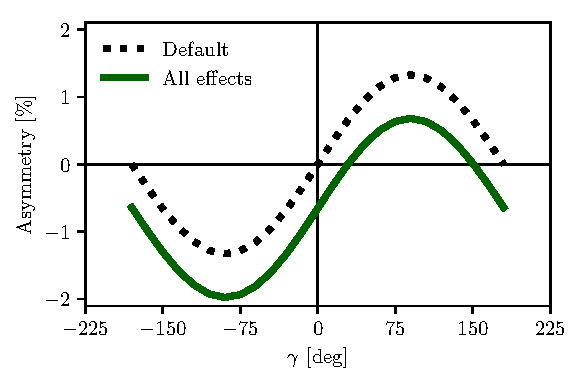
\includegraphics{figures/ks_chapter/paper_asym_for_gammas.pdf}
    \caption{The asymmetry $A_\text{total}$ as a function of $\gamma$ calculated to $O(\epsilon)$ using Eq.~\eqref{eq:global_asym}. The calculation is made using for (black dotted line) the default case where $\Delta h = 0$ and (green) including neutral kaon \CP-violation and material interaction with $r_\chi=\epsilon$.}
    \label{fig:global_asym}
\end{figure}

The second observation relates to potential future measurements of $\gamma$, which may also include sensitivity from the total, phase-space-integrated yield asymmetry
\begin{align}\label{eq:global_asym}
    A_\text{total}=\frac{N^--N^+}{N^-+N^+} = 
    \frac{ 2(2\mathcal F_+ -1)r_B \sin \delta_B \sin \gamma +\Delta h}
    {1 + r_B^2+ 2(2\mathcal F_+ -1) r_B \cos \delta_B \cos \gamma} + O(r\epsilon),
\end{align}
where the definition of $\mathcal F_+$ from Section~\ref{sub:relation_to_glw_and_ads_measurements} has been employed. In the limit $r_B\to 0$ the expression agrees with the result for the analogous asymmetry in $\Dpm\to\pipm\KS$ decays in Ref.~\cite{grossmanCPViolationKSv2012}, evaluated to $O(\epsilon)$ for an infinite and uniform time-acceptance. As hinted at above, the fact that $\mathcal F_+\simeq 0.5$ means that the asymmetry due to $\gamma$ being non-zero is not $\mathcal O(r_B)$, but of approximately the same order of magnitude as the asymmetry due to \CP violation in the neutral kaon sector, governed by $\Delta h$. This is illustrated in Fig.~\ref{fig:global_asym}, where the expression in Eq.~\eqref{eq:global_asym} is plotted in the default case where $\Delta h=0$, using the model in Ref.~\cite{Belle2018} to calculate \Ki and \ci, as well as including neutral kaon \CP violation and material interaction effects, calculated using $r_\chi=\epsilon$, with $\epsilon$ taking the value in Eq.~\eqref{eq:PDG_epsilon}. The asymmetry changes significantly when including the latter effects. Therefore, measurements based only on the global asymmetry will suffer relative biases of tens of degrees, not a few degrees, if neutral kaon \CP violation and material interaction is not taken into account. 


% subsection impact_on_ (end)

% section detector_descriptions_for_lhcb_and_belle_ii (end)

\section{\texorpdfstring{Impact on BPGGSZ measurements of $\gamma$:\\LHCb and Belle II measurements}{Impact on BPGGSZ measurements of gamma: LHCb and Belle II measurements}} % (fold)
\label{sec:impact_on_ggsz_measurements}

The previous section has established that the bias due to neutral kaon \CP violation and material interaction is at the sub-percent level for measurements based on \BtoDK decays, and just a few percent in \BtoDpi decays. Thus, the effects only contribute a manageable systematic uncertainty in the measurement that is the subject of the thesis. However, the expected precision on $\gamma$ measurements will increase significantly in the coming decade, as both the \lhcb~\cite{lhcbcollaborationPhysicsCaseLHCb2019} and Belle II~\cite{kouBelleIIPhysics2019} collaborations expect to make BPGGSZ measurements that measure \g with a precision of 1--3$^\circ$. Therefore a deeper understanding of the expected bias for these specific experiments is important.

This section details a study, where the equations of the previous section are evaluated numerically to all orders, and care is taken to realistically model the experiment specific conditions. The scope of the original analysis, published in Ref.~\cite{KsCPV}, was a stand-alone paper that covers both \lhcb and Belle~II, and which therefore does not rely on full detector simulation. Instead the following approaches are taken to model the necessary input
\begin{itemize}
  \item the experimental time-acceptance is modelled based on the detector geometry and typical neutral kaon momentum spectrum
  \item the material interaction is included, using the material budget information available in the technical design reports on each experiment
  \item both the time-acceptance and material interaction depends on the neutral kaon momentum, for which realistic distributions are estimated using the \texttt{RapidSim} simulation package~\cite{cowanRapidSimApplicationFast2017}.
\end{itemize}
Each input is described in detail in the following sections. The study has been repeated to assign a systematic uncertainty to the \lhcb measurement in Chapter~\ref{ch:5-GGSZ-measurement}, with slight adjustments to match the exact fit setup and with the inputs above extracted from full \lhcb simulation. This is described further in Section~\ref{sub:the_impact_on_coupled_btodk_and_btodpi_measurements}.

\subsection{Detector geometries} % (fold)
\label{sub:detector_geometries}

The \lhcb geometry and sub detectors are described in details in Chapter~\ref{ch:3-detector}. In the \lhcb measurement discussed in Chapter~\ref{ch:5-GGSZ-measurement}, the \KS mesons are reconstructed in the $\pip\pim$ final state and two distinct categories of decay are considered, depending on where in the detector the \KS decay occurs. The categories have very different decay-time acceptance, and therefore  two scenarios are considered for \lhcb:  one in which the decay products of the \KS leave reconstructed tracks in both the silicon vertex detector and downstream tracking detectors (denoted \emph{long-long} or LL), and one in which the decay products of the \KS only leave tracks in the downstream tracking detectors (denoted \emph{down-down} or DD). 

\begin{figure}[tb]
  \centering
  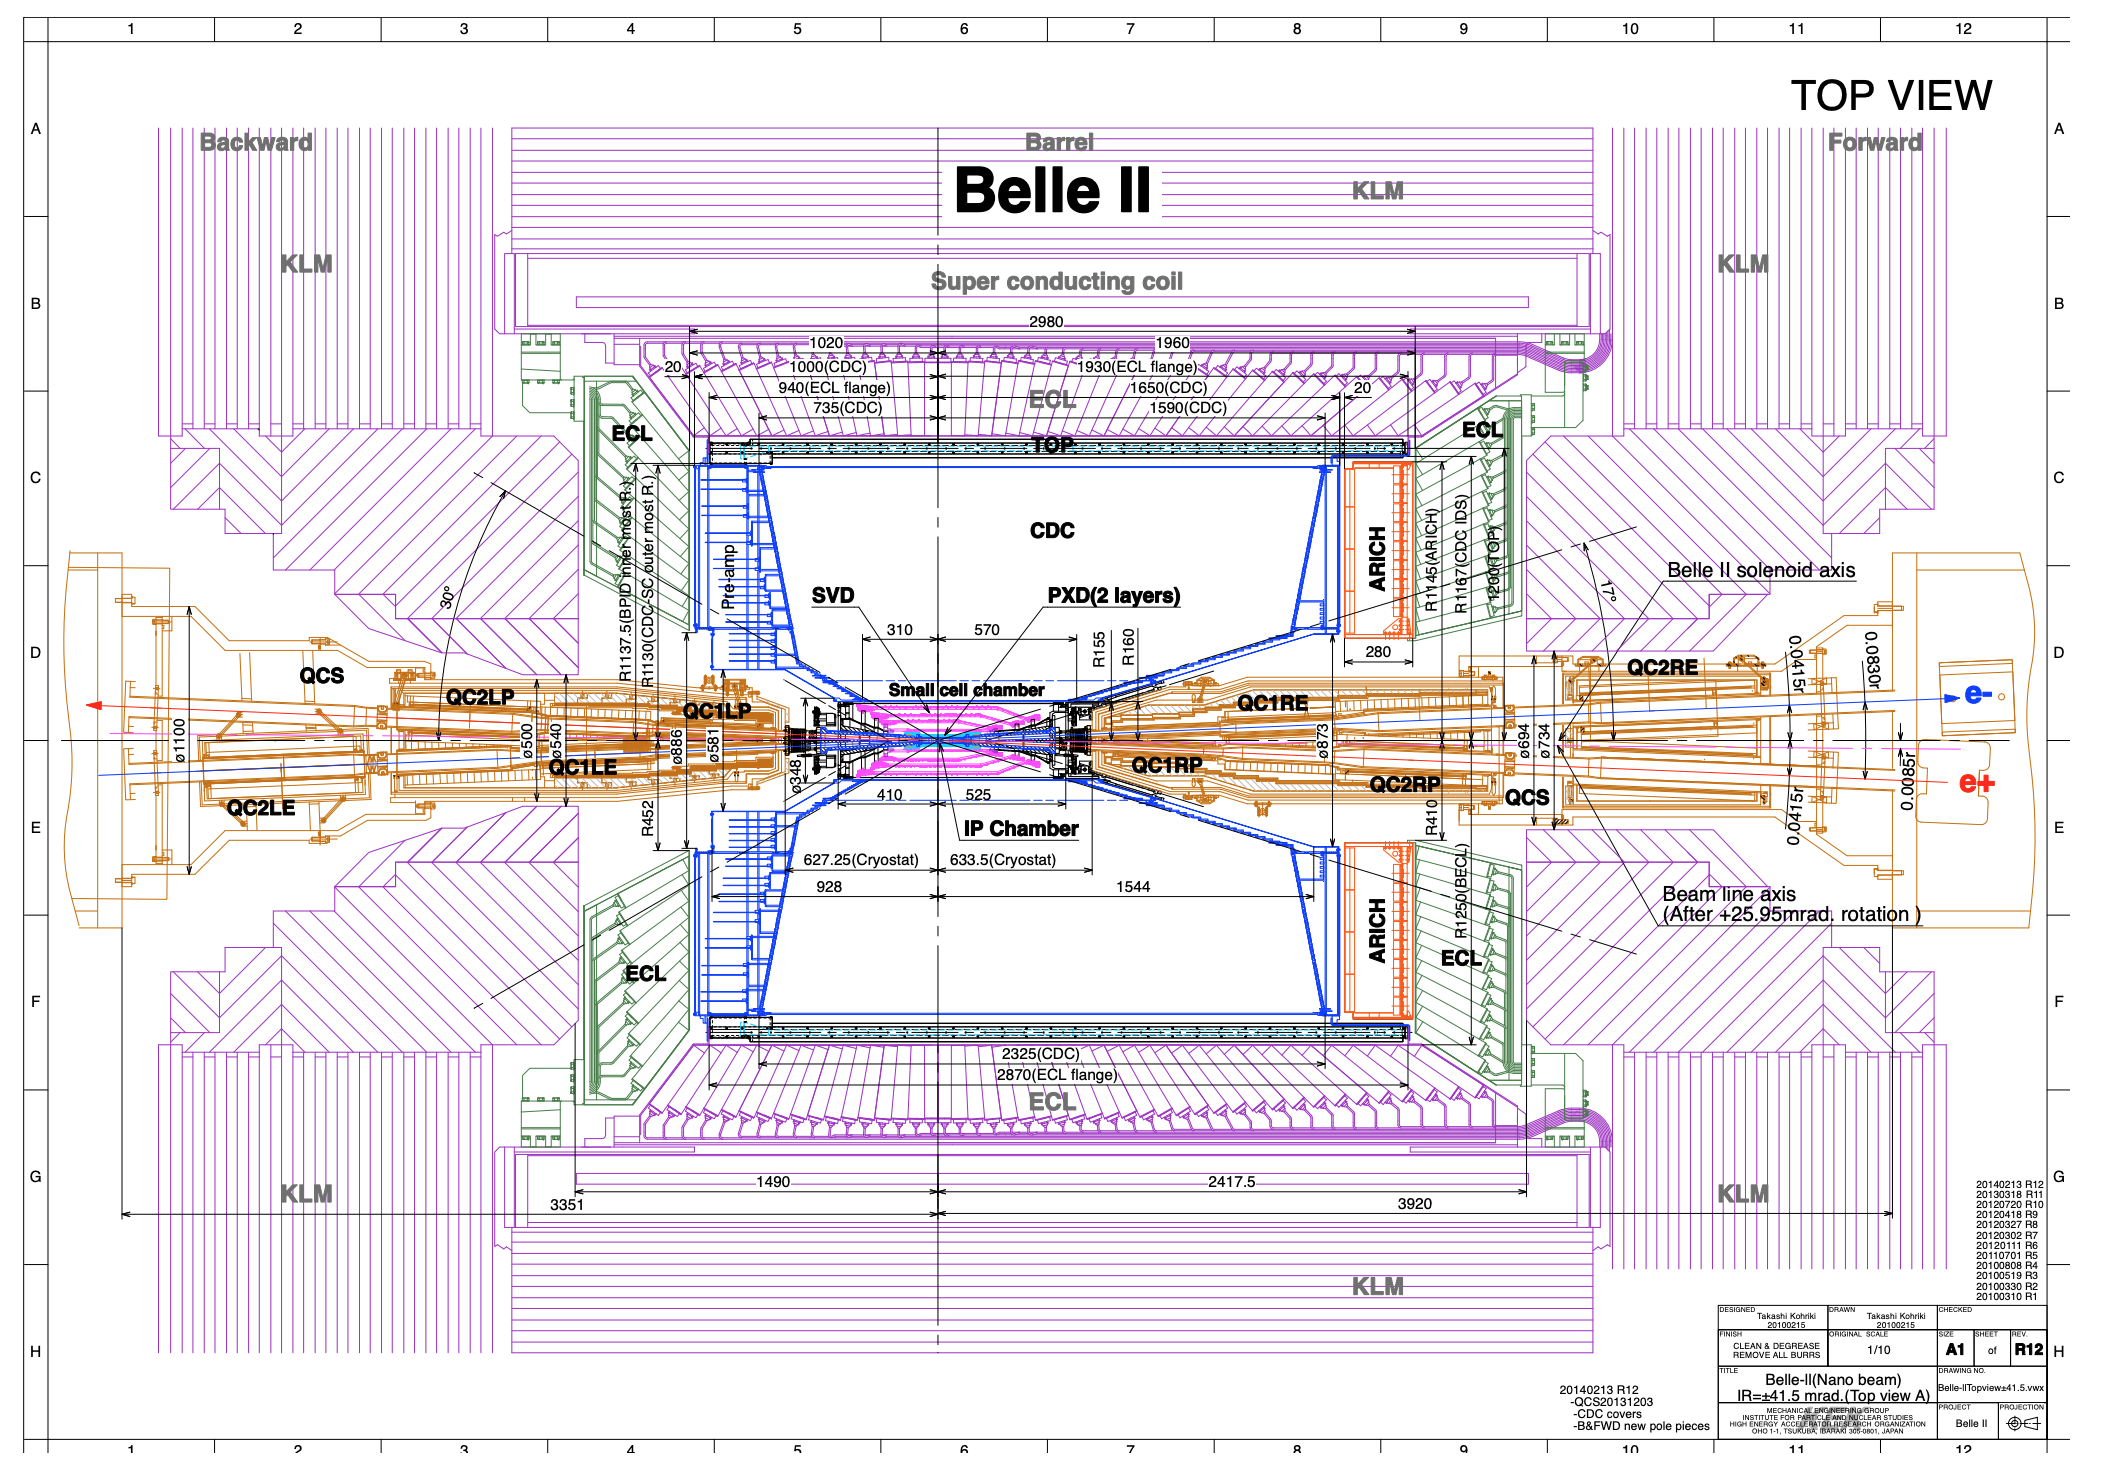
\includegraphics[width=0.8\columnwidth]{figures/ks_chapter/belledetector.png}
  \caption{Schematic of the Belle~II detector, reproduced from Ref.~\cite{kouBelleIIPhysics2019}.}
  \label{fig:belleII_detector}
\end{figure}

The Belle~II detector is a general purpose spectrometer, built to to collect data from asymmetric $e^+e^-$ collisions provided by the SuperKEKB accelerator in Japan~\cite{ohnishiAcceleratorDesignSuperKEKB2013}. A schematic of the detector is shown in Fig.~\ref{fig:belleII_detector}. The relevant sub detectors for the present study are the tracking detectors: a central silicon vertex detector, comprised of a total of six layers within 140\mm of the beam, and a large volume drift chamber with 56 wire layers, extending to a radius of 1130\mm~\cite{kouBelleIIPhysics2019}. 
A single scenario is considered for \belle II, because essentially all the \KS mesons produced in signal decays in Belle II decay within the tracking volume, with more than 90\,\% decaying in the vertex detector according to the studies described below. Thus, three scenarios are considered in total: LL \lhcb, DD \lhcb, and \belle II.

% subsection detector_geometries (end)

\subsection{Kaon momentum distributions} % (fold)
\label{sub:kaon_momentum_distributions}

The neutral kaon momentum distributions are obtained using \texttt{RapidSim}~\cite{cowanRapidSimApplicationFast2017}, a simple tool to generate MC samples. \texttt{RapidSim} has an inbuilt capability to generate decays of \B mesons with the kinematic distribution found in \lhcb collisions and falling in the \lhcb acceptance. However, the distributions need to be reweighted to take the kaon-decay-time acceptance into account. After being reweighted, the \texttt{RapidSim} momentum spectra are reasonably close to those found in full \lhcb simulation samples of $\Bpm\to\D(\to\KS\pip\pim)\Kpm$ decays, as seen in Fig.~\ref{fig:rapidsim_momentum_comparison}


\begin{figure}[tbp]
    \centering
    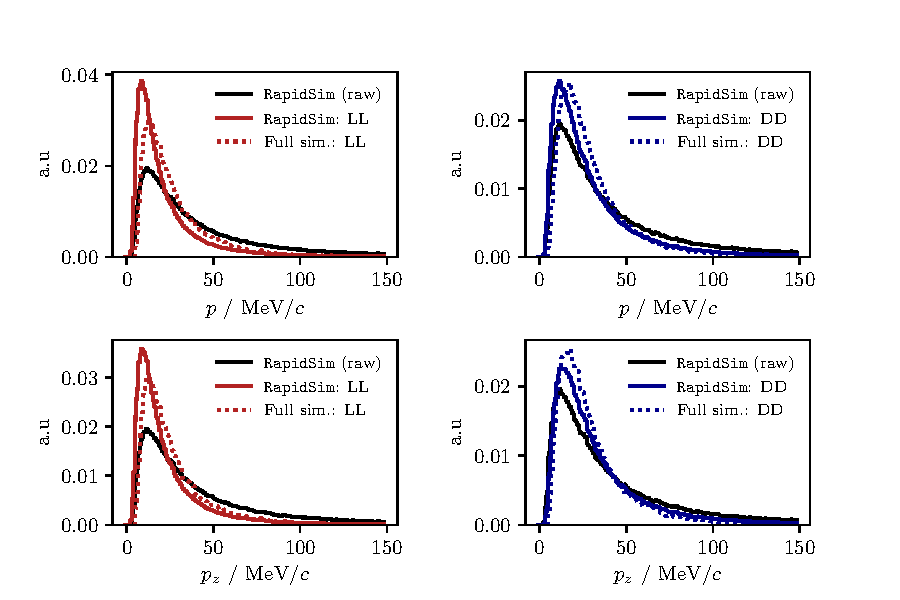
\includegraphics[width=0.98\columnwidth]{figures/analysis/systematics/momentum_distributions_rapidsim_vs_lhcb.pdf}
    \caption{Momentum spectra for the \KS meson in \lhcb, as generated using \texttt{RapidSim} (black lines) directly, as well as reweighed to match decay time acceptance in the (red) LL and (blue) DD data categories of \lhcb. The \lhcb spectra are compared with the spectra in fully simulated signal decays, for both the (dotted red lines) LL and (dotted blue lines) DD data categories.}
    \label{fig:rapidsim_momentum_comparison}
\end{figure}

At \belle II, the signal \B mesons stem from decays of $\Upsilon(4S)$ mesons  produced in asymmetric \text{electron-positron} collisions. This leads to substantially different decay kinematics in comparison to those found at \lhcb. The momentum distribution in \belle II is estimated by letting \texttt{RapidSim} decay \B mesons with a momentum of 1.50 \gevc along the $z$-axis using \texttt{RapidSim}, corresponding to the $\gamma\beta=0.28$ boost of the centre-of-mass system in \belle II when operated at the $\Upsilon(4S)$ resonance~\cite{kouBelleIIPhysics2019}. A perfect $4\pi$ angular acceptance is assumed.   It is not necessary to reweigh the Belle~II momentum spectrum to account for the kaon-decay-time acceptance because all produced \KS mesons decay in the tracking volume. 

The resulting momentum distributions for the three types of sample are shown in Fig.~\ref{fig:momentum}.




\begin{figure}[tbp]
    \centering
    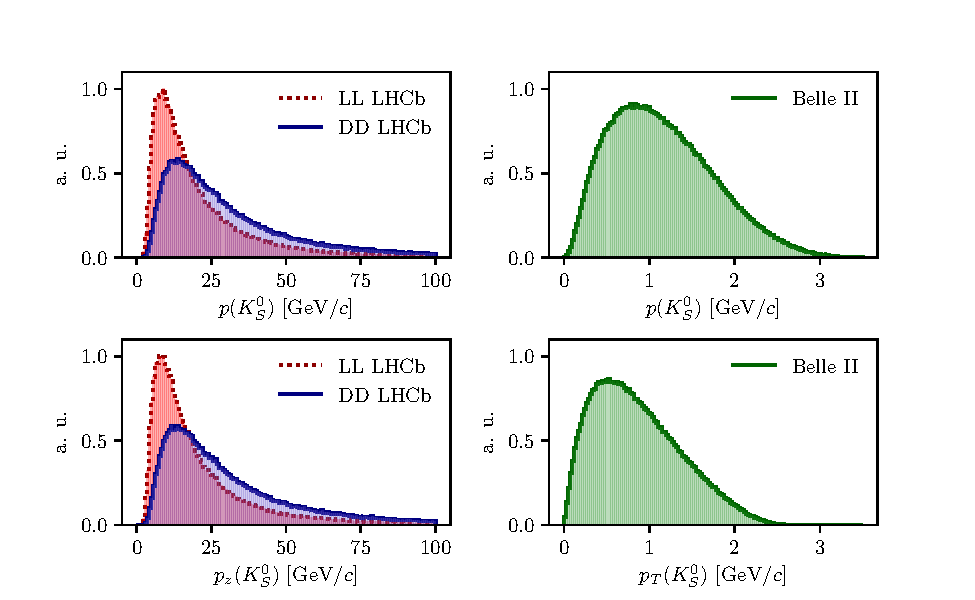
\includegraphics[width=0.98\columnwidth]{figures/ks_chapter/momentum_distributions.pdf}
    \caption{Momentum distributions for the \lhcb (red dotted line) LL and (blue) DD categories, as well as (green) \belle II, obtained using \texttt{RapidSim}.}
    \label{fig:momentum}
\end{figure}


% subsection kaon_momentum_distributions (end)

\subsection{Experimental time acceptance} % (fold)
\label{sub:experimental_time_acceptance}

In order to model the experimental time acceptance, the time-dependent decay rates are only integrated over a finite time interval $(\tau_1, \tau_2)$. The intervals are defined for each of the three experimental categories, by requiring that a neutral kaon, if produced at $x=y=z=0$ with momentum $p=(p_T, p_z)$, decays within the relevant part of the corresponding detector. For the LL \lhcb category, it is required that the kaon decays before reaching $z_{max}=280\mm$, corresponding to a decay where the decay products traverse at least 3 VELO segments (ignoring a number of widely spaced VELO segments placed at a distance of up to $z=750\mm$ from the interaction point)~\cite{CERN-LHCC-2003-030}. For the DD \lhcb category a decay at $z\in[280,2350]\mm$ is required, corresponding to decay between the LL cut-off and the first downstream tracking station~\cite{LHCb-2003-140}. 
%The decay-time distribution using these cutoff values are compared that found in full \lhcb simulation in Fig.~\ref{fig:dec_time_dist}. It is found to be reasonably good, especially in the DD category. In the LL category, the physical cut-off is less well-defined, because the $z$ position of the last VELO tracking segment a given track intersects depend on the angle with the beam line. In the studies used to assign a systematic uncertainty on the \lhcb measurement in Chapter~\ref{ch:5-GGSZ-measurement}, a better acceptance model was employed, defined with a soft turn-on based on full \lhcb simulation. The expected decay-time distribution assuming this acceptance function is also shown in Fig.~\ref{fig:dec_time_dist}.
The time acceptance has a significant impact for the \lhcb categories, where some 20\,\% of the kaons escape the tracking stations completely before decaying.

% \begin{figure}[tb]
%     \centering
%     \begin{subfigure}{\columnwidth}\centering
%         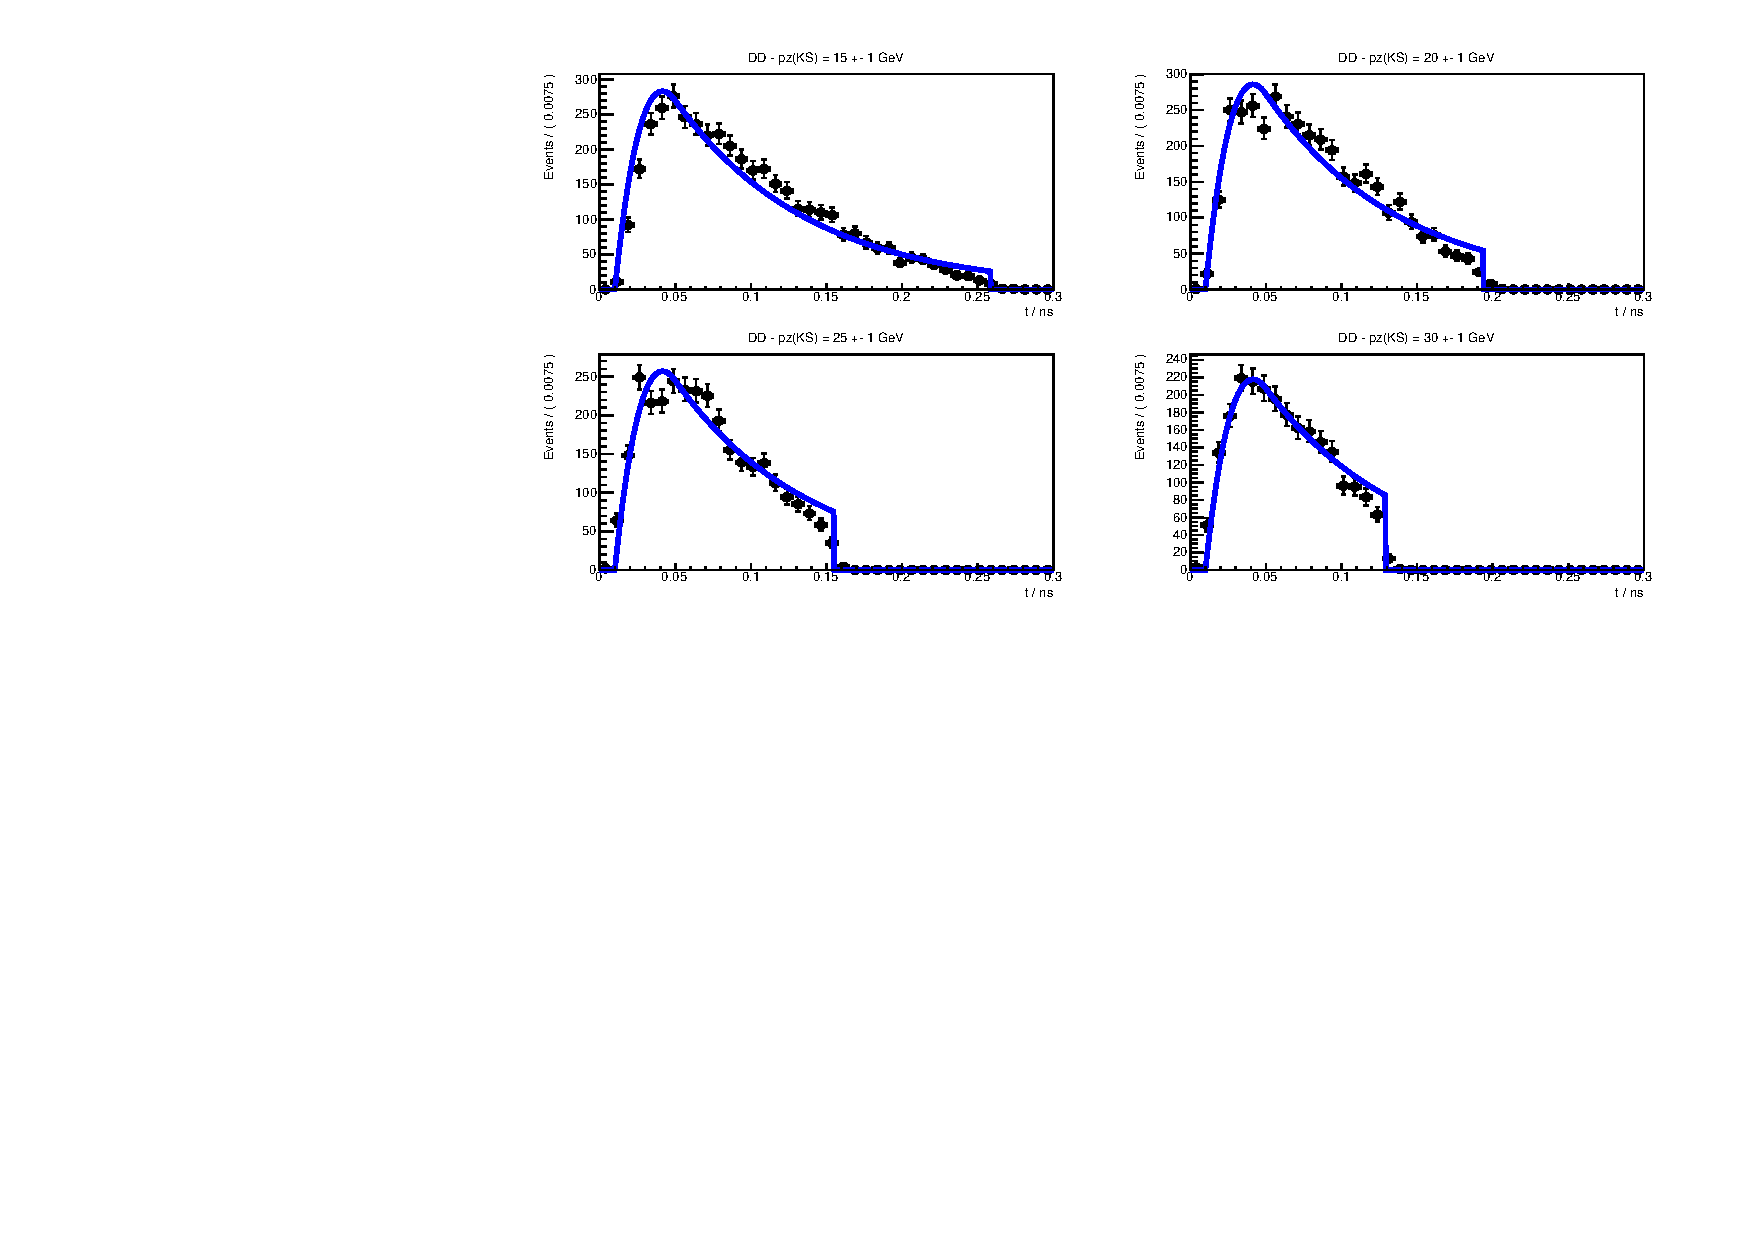
\includegraphics[width=0.8\columnwidth]{figures/ks_chapter/note_figs/lhcb_studies/1d_DD_time_acceptance_result.pdf}
%         \caption{}\label{fig:dec_time_dist_DD}
%     \end{subfigure}
%     \begin{subfigure}{\columnwidth}\centering
%         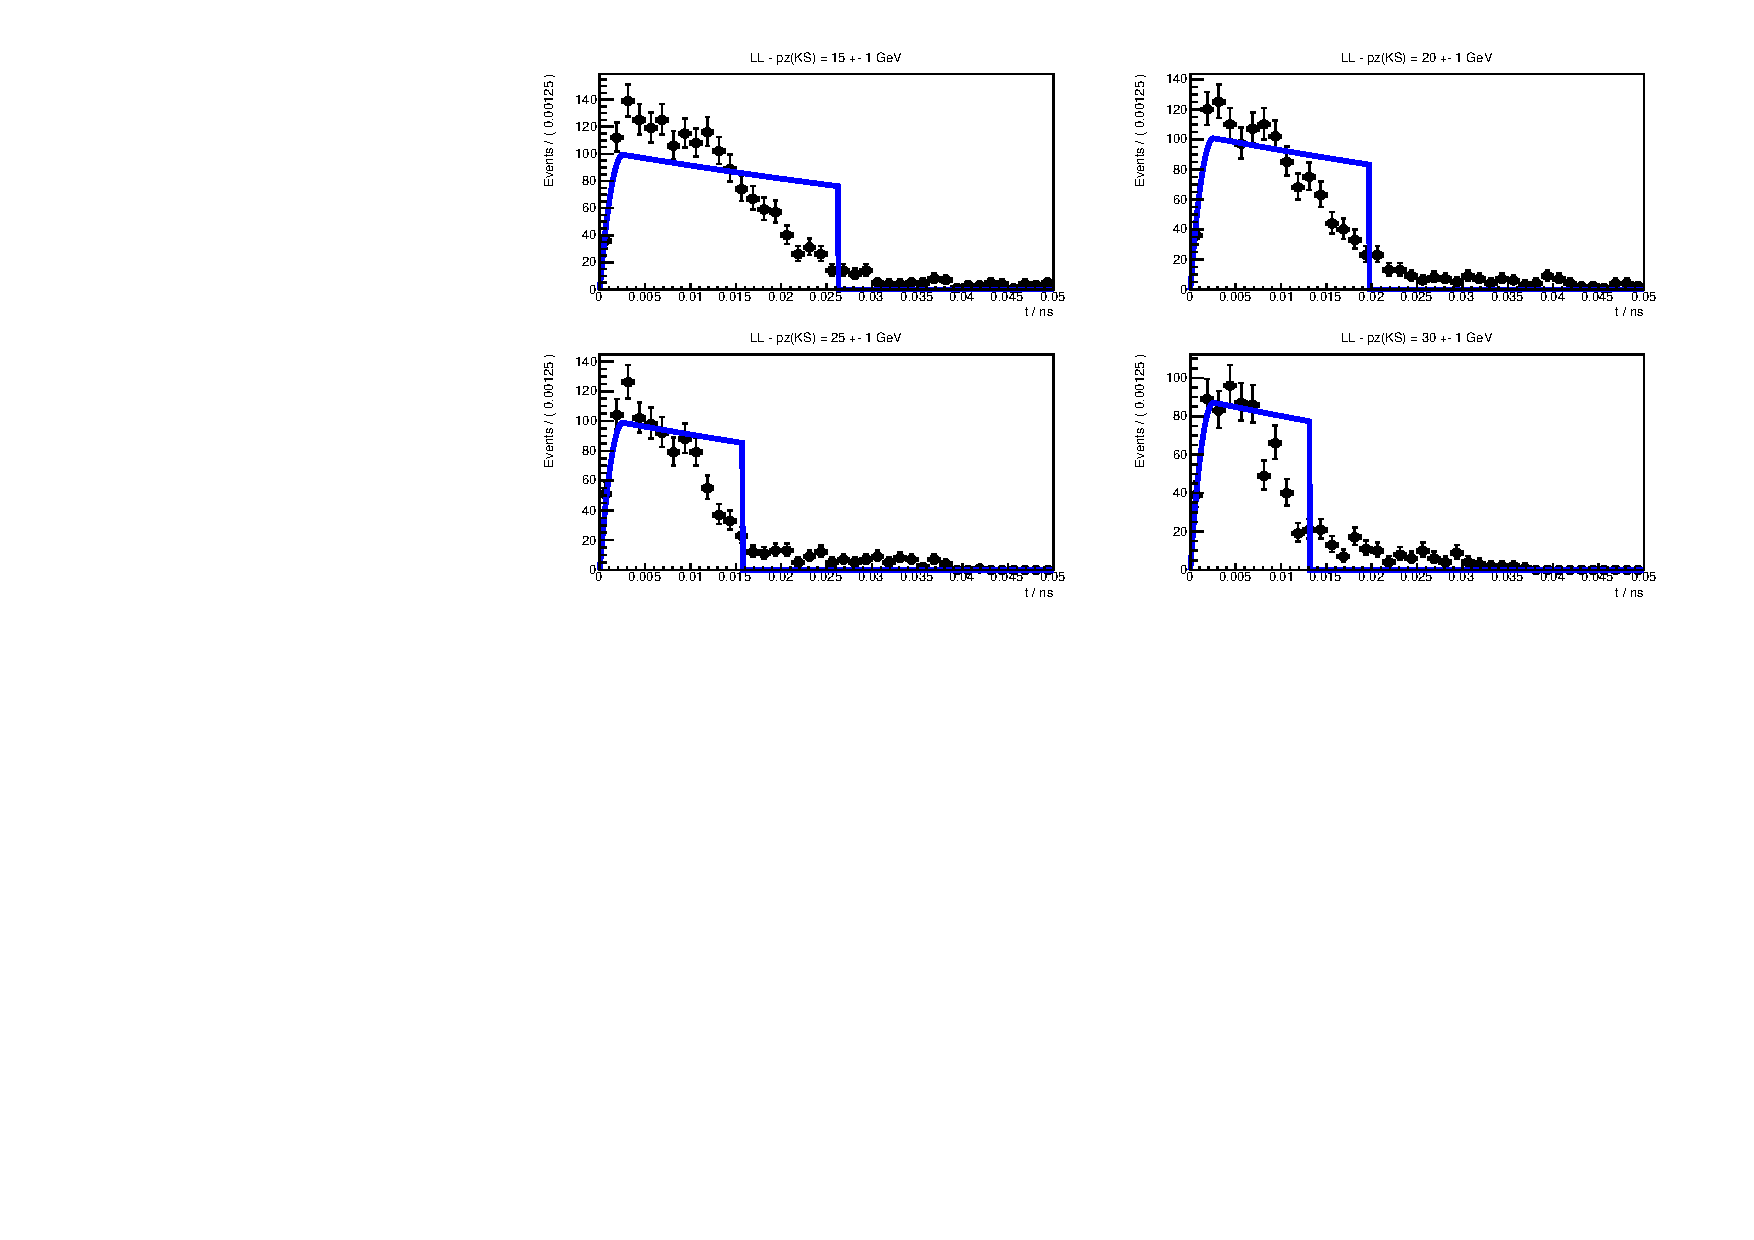
\includegraphics[width=0.8\columnwidth]{figures/ks_chapter/note_figs/lhcb_studies/1d_LL_time_acceptance_result.pdf}
%         \caption{}\label{fig:dec_time_dist_LL}
%     \end{subfigure}
%     \caption{Decay time distribution of simulated \lhcb signal decays in the (top) DD and (bottom) LL data categories, for four different, narrow $p_z(\KS)$ regions. The expected distributions given the time acceptance used in the simple studies  are overlaid.\label{fig:dec_time_dist}} 
% \end{figure}

For \belle II, it is assumed that the \KS reconstruction is similar to {}the \belle\ \KS reconstruction, which is based on a neural network and reconstructs \KS decays for which the decay product leave tracks in both the drift chamber and silicon vertex detectors, as well as decays that leave tracks in the drift chamber only~\cite{BelleKSPaper,BelleKSThesis}. Therefore, the \KS decay is required to be within $r_{max}=1130\mm$ of the beam axis, corresponding to a decay within the outer radius of the drift-chamber. In practice, most of the kaons already decay inside the silicon vertex detector, and requiring a decay before the outer radius of the drift chamber is essentially equivalent to having no time cut-off.



% subsection experimental_time_acceptance (end)

\subsection{Detector material budget} % (fold)
\label{sub:detector_material_budget}

The effect of the material interaction is governed by parameter $\Delta\chi$ of Eq.~\eqref{eq:mat_param}. The parameter varies along a given kaon path, as the kaon intersects detector components made of different materials. In these studies, the calculations are simplified by using a single average material parameter for each experimental scenario. The average material parameters can be estimated for a given experimental scenario by considering the type and length of material traversed by a kaon in the relevant sub-detector(s). The average value is estimated, by exploiting that $\Delta\chi$ is related to the forward scattering amplitude $f$ $(\bar f)$ of \Kz (\Kzb) mesons in a given material~\cite{goodRelationScatteringAbsorption1957,fetscherRegenerationArbitraryCoherent1996}
\begin{align}\label{eq:mat_delta_chi}
    \Delta \chi = - \frac{2\pi \mathcal{N}}{m_K}(f-\bar f) = - \frac{2\pi (N_A \rho/A)}{m_K}(f-\bar f),
\end{align}
where $\mathcal{N}=N_A\rho/A$ is the scattering centre density of the material, $m_K$ is the mass of the kaon state,  $A$ and $\rho$ are the nucleon number and density of the material, and $N_A$ is Avogadro's number.
Measurements made for a range of nuclei~\cite{Gsponer1979} show that in the momentum range $p_K\in [20, 140]\gevc$
\begin{align} \label{eq:f_p_dep}
    \left|\frac{f-\bar f}{p_K}\right| = 2.23 \frac{A^{0.758}} {p_K^{0.614} (\gevc)} \text{ mb}, \quad \arg [f - \bar f] = -\frac{\pi}{2}\left(2-0.614\right),
\end{align}
where the phase of $\Delta f$ is determined via a phase-power relation~\cite{Briere1995}. In the numerical studies presented here, Eq.~\eqref{eq:f_p_dep} is also used for the low momentum neutral kaons in the \belle II calculations, as a more detailed modelling of the low momentum $\Delta\chi$ based on Ref.~\cite{Ko2011} is found to yield very similar results. The scattering centre density $\mathcal{N}$ is approximated as being constant, equal to the average density along a neutral kaon path due to its intersection with different detector segments. This average is estimated using the simplifying assumption that the total detector material budget is due to silicon. In practice, $\mathcal{N}=N_A\rho/A$ is calculated using $A=28$ and $\rho = f^\text{Si}\rho^\text{Si}$, where $f^\text{Si}<1$ is the average fraction of a neutral kaon path length that is inside detector material, estimated via the known dimensions of the detector, the average nuclear interaction length seen by a track traversing it cf. the technical design reports~\cite{CERN-LHCC-2003-030,RICH-TDR}, and the nuclear interaction length of silicon $\lambda_I^\text{Si}=465.2\mm$~\cite{PDG2020}. 
The average value of $r_\chi=\frac{1}{2}\frac{\Delta\chi}{\Delta\lambda}$, which governs the size of the matter regeneration effect, can be calculated for the three considered experimental scenarios and satisfy $|r_\chi^\text{LL}|=2.7\times10^{-3}$, $|r_\chi^\text{DD}|=2.2\times10^{-3}$, and ${|r_\chi^\text{Belle II}|=1.0\times10^{-3}}$. 

The neutral kaon tracks in \lhcb generally pass through somewhere between zero (for a significant amount of the LL tracks) and a hundred (for some DD tracks) distinct detector segments. Therefore it is worth examining the degree to which using a single average $\Delta\chi$ value, obtained following the procedure outlined above, provides a reasonable description of the average material interaction. This can be done using full \lhcb simulation, where the kaon state for a simulated track can be evaluated at all times, by applying Eq.~\eqref{eq:mat_time_dep} iteratively for each detector segment the track traverses, using a $\Delta\chi$ value appropriate for that segment. 
%The results can then be compared to those obtained using a single average $\Delta\chi$. 
This is done in Fig.~\ref{fig:lhcb_asymmetry} for a simple observable: the yield asymmetry 
\begin{align}\label{eq:KKb_asymmetry_definition}
    A_{K^0} = \frac{|\psi_\Kz(t)|^2 - |\psi_\Kzb(t)|^2}{|\psi_\Kz(t)|^2 + |\psi_\Kzb(t)|^2},
\end{align}
where $\psi_\Kz(t)$ ($\psi_\Kzb(t)$) is the amplitude for an initial \Kz (\Kzb) to decay to two pions at time $t$. In this calculation, it is assumed that $\epsilon=0$ to isolate the material effect with no asymmetry contribution from the inherent \CP-violation in the neutral kaon sector. While the track-by-track asymmetries are found to differ significantly depending on the exact detector segments a track intersects, the average asymmetry is seen to evolve smoothly as a function of decay time, and in reasonable agreement with the asymmetry value that is calculated using the average $\Delta\chi$ values estimated above. 


\begin{figure}[tb]
    \centering
    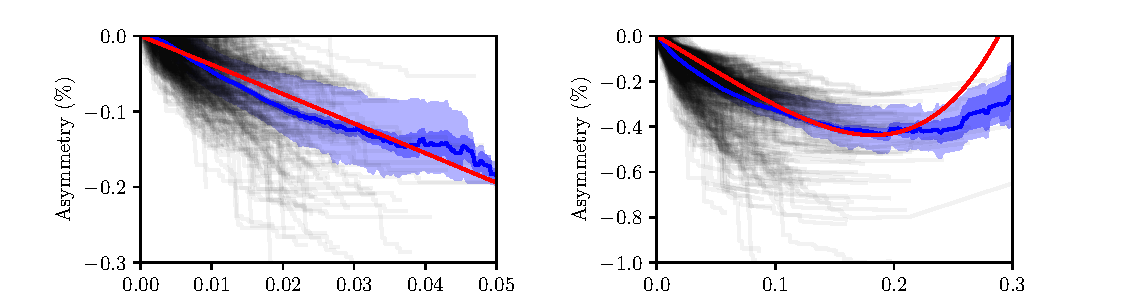
\includegraphics[width=\columnwidth]{figures/analysis/systematics/compare_material_int_asym.pdf}
    \caption{The asymmetry in Eq.~\eqref{eq:KKb_asymmetry_definition} as a function of time for \KS tracks in samples of simulated (left) LL and (right) DD decays, using the full \lhcb simulation. The light blue area is the central 50 \% quantile of all tracks, the dark blue area is the 1$\sigma$ uncertainty band on the mean. The black lines show the result for a subset of individual, randomly sampled tracks. The red lines are calculated using the average $\Delta\chi$ values that are also used in the calculation of biases in BPGGSZ measurements.}
    \label{fig:lhcb_asymmetry}
\end{figure}



The \lhcb detector is undergoing a significant upgrade prior to the start of the LHC Run~3. However, the material budget and geometry of the relevant sub-detectors will be similar to the sub-detectors used during Run~1~and~2~\cite{VELOUpgradeTDR,PIDUpgradeTDR}. Hence the results of this study will be valid for measurements during the upgrade phases of \lhcb, even though the detector parameters presented in this section relate to the original \lhcb detector.

% subsection detector_material_budget (end)

\subsection{Calculation procedure} % (fold)
\label{sub:calculation_procedure}

The main idea in the bias study is to calculate the BPGGSZ bin yields including the full effect of neutral kaon \CP violation and material, fit them using the default equations of Chapter~\ref{ch:2-litreview}, and thereby obtain the bias $\Delta\gamma = \gamma - \gamma^0$ due to the kaon effects not being considered in the parameter extraction. For the purpose of Ref.~\cite{KsCPV}, a simple fit setup of a single \BtoDh mode is investigated, where the \Ki parameters are determined in a control channel with the relevant experimental acceptance. This setup is modified in the study used to assign a systematic uncertainty on the \lhcb measurement of Chapter~\ref{ch:5-GGSZ-measurement}, as described in Section~\ref{sub:the_impact_on_coupled_btodk_and_btodpi_measurements} below.


In practice, the amplitude model for $\Dz\to\KS\pip\pim$ decays in Ref.~\cite{Belle2018} is taken to represent the $A_1(\spm)$ amplitude. Then $A_2(\spm)$ is obtained as described in Section~\ref{sub:relationship_between_the_ks_and_kl_amplitudes}. In terms of $A_1$ and $A_2$, the amplitudes $\ADorDbSL(\spm)$ can be expressed and related via Eqs.~\eqref{eq:A12toKS}~and~\eqref{eq:DDbar_relations}, and the full signal decay amplitudes as a function of phase-space coordinates, time, and the material interaction parameter $\Delta\chi$ can be calculated for a given set of input parameters $(\gamma^0, r_B^0, \delta_B^0)$. The squared decay amplitudes are then integrated over phase space and the kaon decay times to obtained the binned signal yield.

The signal yields depend on the momentum via the time-acceptance parameters $\tau_1$ and $\tau_2$, and because the material interaction parameter $\Delta\chi$ is momentum dependent. Therefore, the yields are averaged over the \KS momentum distributions of \lhcb and \belle II. 


The parameters \xpm and \ypm are determined by a maximum likelihood fit to the calculated yields, after which the fit result and covariance matrix are interpreted in terms of the physics parameters $(\gamma, r_B, \delta_B)$ using another maximum likelihood fit~\cite{LHCb-PAPER-2016-032}. In the fits, the $K_i$ are obtained using the definition $K_i=K_i^\text{meas}=({N^\D_i + N^\Dbar_{-i}})/({\sum_j N^\D_j +N^\Dbar_{-j}})$, in terms of the expected yields $N^\D_i$ ($N^{\Dbar}_i$) of a flavour-tagged \Dz (\Dzb) decays in bin $i$ of the \D decay phase space, calculated as described above for $r_B^0=0$. This corresponds to experimentally measuring the $K_i$ in a control channel, and takes the effect of neutral kaon \CP violation and material interaction on $K_i$ measurements into account, as well the experimental time acceptance. The $(c_i, s_i)$ are calculated using $A_1(\spm)$ and the experimental time acceptance is taken into account in this calculation as well. 



% subsection calculation_procedure (end)




 











\subsection{Results} % (fold)
\label{sub:bias_results}


\begin{figure}[tbp]
    \centering
    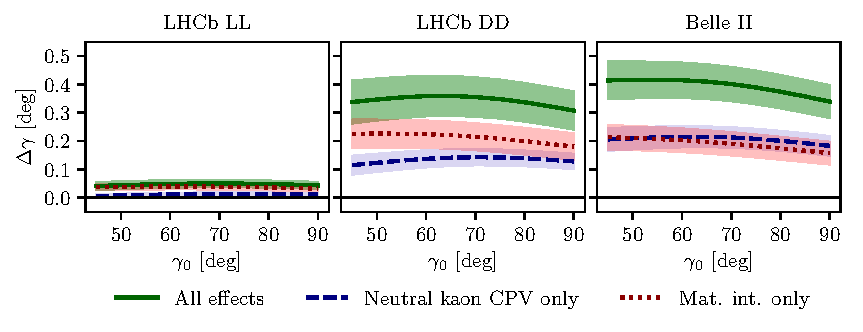
\includegraphics{figures/ks_chapter/gamma_scan_Belle2018_50_g.pdf}
    \caption{The bias $\Delta \gamma$ as a function of input $\gamma_0$ for (left) the LL \lhcb category, (centre) the DD \lhcb category, and (right) \belle II. The bias is calculated due to (blue, dashed line) neutral kaon \CP violation alone, (red, dotted line) material interaction alone, and (green line) both effects. The shaded region shows the estimated $1\sigma$ uncertainty band.}
    \label{fig:compare_experiments}
\end{figure}


The obtained bias $\Delta\gamma$ is shown as a function of input $\gamma^0$ for the various experimental conditions in Fig.~\ref{fig:compare_experiments}. The calculations are made using $(r_B^0, \delta_B^0)=(0.1, 130^\circ)$, approximately equal to the physics parameters relevant for $\Bpm\to\D\Kpm$ decays~\cite{UTfit-UT,HFLAV}.  The bias does not vary significantly with $\gamma^0$ in the plotted range, which includes the world average value of direct $\gamma$ measurements as well as the values obtained in full unitarity-triangle fits~\cite{HFLAV,UTfit-UT,CKMfitter2015}, and for all cases, the bias is found to be below $0.5^\circ$, corresponding to relative biases of about half a percent. Thus the biases are of $O(r\epsilon /r_B)$ as expected, given the arguments of Section~\ref{sub:modification_of_the_bpggsz_yield_equations}. The contributions from the individual \KS CPV and material interaction effects are also shown. It is seen that the neutral kaon \CP violation and material interaction effects leads to approximately equal biases in all three cases. 

Given the decay-time acceptance and momentum distribution for each experimental category, the mean life time, $\langle\tau\rangle$, of the reconstructed kaons can be calculated. In terms of the \KS lifetime ${\tau_\KS=(0.895\pm0.004)\times10^{-11}\,}$s~\cite{PDG2020}, $\langle\tau_\text{LL}\rangle\simeq0.1\tau_\KS$ for the \lhcb LL category, $\langle\tau_\text{DD}\rangle\simeq0.8\tau_\KS$ for the \lhcb DD category, and at \belle II $\langle\tau_\text{Belle II}\rangle\simeq\tau_\KS$. The difference in average kaon lifetime is reflected in the observed biases, which are found to be larger in the samples with longer lived kaons. The very small effect in the LL category is to be expected because the \CP-violation effect due to \KS not being \CP-even is approximately cancelled by the \CP-violation effect arising from $\KS-\KL$ interference for kaons with decay times much smaller than $\tau_\KS$~\cite{grossmanCPViolationKSv2012}. 
%The time dependence of the bias effect means that it can potentially be beneficial to restrict a measurement to using short-lived \KS mesons in a future scenario, where the impact of \KS\ \CP violation is comparable to the statistical precision of the measurement. For example, the bias can reduced by 40\,\% in the \belle II scenario if only \KS mesons decaying within 8\cm of the beam axis are included in the measurement. This requirement only removes 20\,\% of the signal yield, and hence only increases the statistical uncertainty of the measurement by 10\,\%.

The uncertainty bands in Fig.~\ref{fig:compare_experiments} are calculated by repeating the study while varying some of the inputs. The model dependence of the predicted biases is probed by repeating the study using two other amplitude models as input for $A_1(\spm)$ and $A_2(\spm)$: the model published in Ref.~\cite{BELLE2010} and the model included in \sc{EvtGen}\normalfont~\cite{EvtGen}. 
%The use of different models change the predicted biases by up to $0.05^\circ$. W
then defining $A_2(\spm)$ in terms of $A_1(\spm)$, there is an uncertainty due to the unknown $(r_k, \delta_k)$ parameters used to describe the $\pi\pi$ resonance terms. This uncertainty is assessed by making the study with several different random realisations of the parameter set. 
%The phases $\delta_k$ are sampled uniformly in the interval $[0, 2\pi]$ while the $r_k$ are sampled from a normal distribution with $\mu=\tan^2\theta_C$ and $\sigma=\mu/2$. The uncertainty is about $0.05^\circ$ across the three experiments considered. 
The studies are repeated while varying the time acceptances and material densities with $\pm 10\,\%$. 
%The largest deviations in biases are found to be below $0.05^\circ$. The dependence on the handling of the momentum distribution is estimated by repeating the study using 10 and 20 quantiles to describe the momentum distributions at each point in phase space, instead of 5. The variation in the results is taken as the systematic uncertainty, and found to be below $0.01^\circ$ for all experiments. 
There is an additional uncertainty due to the use of simulation samples generated with \texttt{RapidSim} to describe the kaon momentum distribution, in lieu of full detector simulations. 

There is also an uncertainty from the use of $(\ci, \si)$ as calculated using $A_1(\spm)$. It is to be expected that the measured values $(\hat c_i, \hat s_i)$ from the \cleo collaboration differ by those calculated using $A_1^D(s_-,s_+)$ by terms of $O(\epsilon)$ due to neutral kaon \CP violation, which is not taken into account in the measurement~\cite{CLEOCISI}. These corrections can be calculated via a procedure analogous to the one used to estimate the corrections on measurements of $\gamma$ in this paper. However, as these corrections are much smaller than the experimental uncertainties in the measurement, they have not been studied further.

%It is interesting to evaluate the bias obtained if the \Ki are calculated from $A_1(\spm)$, without any corrections due to neutral kaon \CP violation and material interaction. If this is done, while the full experimental time acceptance is taken into account, the biases only change by up to $0.01^\circ$, across the experiments. This is because the $O(\epsilon)$ corrections in Eq.~\eqref{eq:hat_Ki}, where the expected measured \Ki is given to lowest order in $\epsilon$ and $r_\chi$, only affect the overall normalisation. If the time acceptance \emph{is not} taken into account, biases of several degrees can occur, irrespective of the presence of neutral kaon \CP violation or material interaction effects. 


\begin{figure}[tbp]
    \centering
    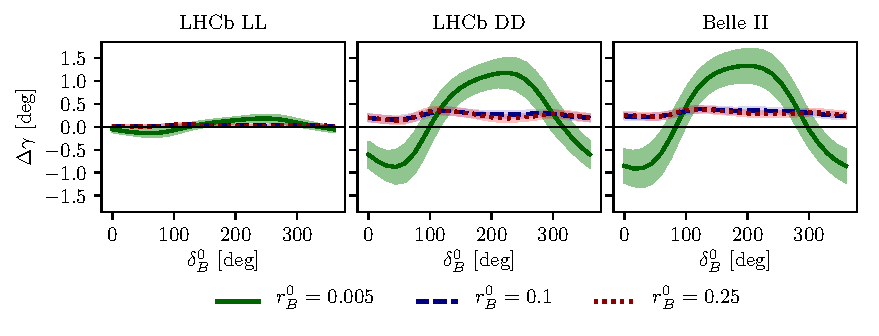
\includegraphics{figures/ks_chapter/delta_scan_Belle2018_50_g.pdf}
    \caption{The bias $\Delta \gamma$ as a function of input $\delta_B$ for (left) the LL \lhcb category, (centre) the DD \lhcb category, and (right) \belle II. The bias is calculated for $\gamma=75^\circ$ and (green line) $r_B=0.005$, (blue, dashed line) $r_B=0.1$, and (red, dotted line) $r_B=0.25$. The shaded region shows the estimated $1\sigma$ uncertainty band.}
    \label{fig:delta_scan}
\end{figure}


For the purpose of this thesis, it is important to consider the bias in measurements that use \BtoDpi decays as well, and other \B decay modes can also be used in BPGGSZ measurements, such as $\Bpm\to\Dstar\Kpm$, $\Bpm\to\D\Kstarpm$, and $\Bz\to\D\Kstarz$. For the purpose of the study presented here, the main difference between the decay channels is that they have different values of $r_B$ and $\delta_B$. Figure~\ref{fig:delta_scan} shows $\Delta\gamma$ as a function of input $\delta_B^0$, for $\gamma^0=75^\circ$ and three different values of $r_B^0$. Aside from $r_B^0=0.1$, the results are shown for $r_B^0=0.005$, which corresponds to the expectation in $\Bpm\to\D\pipm$ decays~\cite{rDpi} and $r_B^0=0.25$, which corresponds to $\Bz\to\D\Kstarz$ decays~\cite{LHCb-CONF-2018-002}. The most notable feature is that the biases are significantly larger in the \BtoDpi case. This is expected: the $r^0_B$ dependent behaviour is governed by the relative importance of different $O(r\epsilon)$ correction terms to the phase-space distribution. There are terms of both $O(r_A\epsilon)$ and $O(r_B\epsilon)$\footnote{There are similar terms of $O(r_Ar_\chi)$ and $O(r_Br_\chi)$, but as $\epsilon$ and $r_\chi$ are of the same order of magnitude, these terms can be treated completely analogously to the $O(r_A\epsilon)$ and $O(r_B\epsilon)$ terms, and have been left out of the discussion for brevity.}, which lead to expected biases of size $O(r_A\epsilon/r_B)$ and $O(r_B\epsilon/r_B)=O(\epsilon)$, respectively, cf. the discussion of Section~\ref{sub:modification_of_the_bpggsz_yield_equations}. 
In the $\Bpm\to\D\pipm$ case, the $O(r_A\epsilon)$ correction terms dominate because $r_A/r_B\simeq (0.05/0.005)=10$. This explains the relatively large bias, as $|r_A\epsilon/r_B^{D\pi}|\simeq 4\%$. The bias is seen to be up to {}$\pm1.5^\circ$, but only about $+0.2^\circ$ with the expected value of $\delta_B^{D\pi}\simeq300^\circ$~\cite{LHCb-PAPER-2016-032,rDpi}. These biases are \emph{much smaller} than the precision on $\gamma$ that is obtainable in a \BtoDpi analysis with current experimental yields, and do thus not pose a problem.
In the $r_B^0=0.1$ and $r_B^0=0.25$ cases the $O(r_B\epsilon)$ correction terms dominate, and the biases are of $O(\epsilon)$, independent of the $r_B^0$ value. Therefore both cases have biases of similar size.



Further, it is clear that the biases depend on $\delta_B^0$ and that the oscillation period of the $\delta_B$ dependence is different between the $r^0_B=0.005$ case and the $r_B^0\in\{0.1, 0.25\}$ cases. It is to be expected that $\Delta\gamma$ oscillates as a function of $\delta^0_B$, because $\delta_B^0$ enters the yield equations via $\cos(\delta_B^0\pm\gamma)$ and $\sin(\delta_B^0\pm\gamma)$ terms.  As explained above, the $O(r_A\epsilon)$ terms dominate the \BtoDpi bias, and these are independent of $\delta_B^0$. The $O(r_B\epsilon)$ terms, however, are important for the bias corrections for larger $r_B$ values, and the terms include factors of $\cos(\delta_B^0\pm\gamma)$ and $\sin(\delta_B^0\pm\gamma)$. This explains the different bias dependence on $\delta^0_B$. 


While the input value of $\gamma^0=75^\circ$ was chosen for these studies, there is minimal variation in the results if another value of $\gamma^0$ in the range $[60^\circ, 85^\circ]$ is used.


\subsection{\texorpdfstring{Coupled \BtoDK and \BtoDpi measurements}
{Coupled B->DK and B->Dpi measurements}}% (fold)
\label{sub:the_impact_on_coupled_btodk_and_btodpi_measurements}

The studies presented above have been extended on two accounts in order to assign a systematic uncertainty to the \lhcb measurement presented in Chapter~\ref{ch:5-GGSZ-measurement}. Firstly, full \lhcb simulation has been used to obtain the momentum distributions, as well as to fit a better description of the time acceptance and the reconstruction efficiency profile over the \D-decay phase space. Secondly, the fit setup is modified to correspond to the experimental approach described in Section~\ref{sec:strategy_for_lhcb_measurement} and Chapter~\ref{ch:5-GGSZ-measurement}: the signal yields are calculated for both the \BtoDK and \BtoDpi channels, and fitted in a combined fit to obtain $(\xpmdk, \ypmdk, \xxidpi, \yxidpi)$, where the \Fi parameters are allowed to float in the fit. The biases obtained for each observable are shown in Fig.~\ref{fig:LHCb_related_biases}, evaluated using the time-acceptance, momentum distribution, and material budget relevant for the DD category (since the effect in the LL category is much smaller). As will be clear in Chapter~\ref{ch:5-GGSZ-measurement}, these biases are all significantly smaller than the corresponding statistical uncertainties. Thus, the effects of neutral kaon \CP violation and material interactions contribute a manageable systematic uncertainty in current BPGGSZ measurements, even if the \BtoDpi channel is promoted to a signal channel.

\begin{figure}[tb]
  \centering
  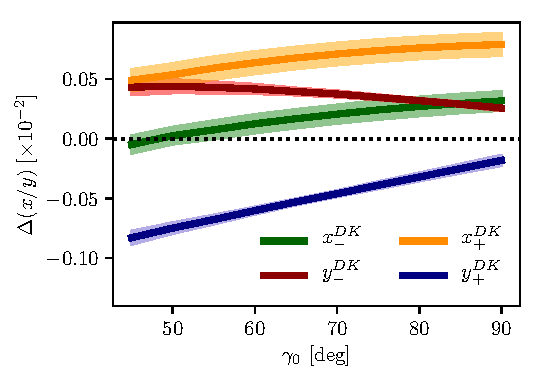
\includegraphics[width=0.45\columnwidth]{figures/ks_chapter/delta_xy_dk.pdf}
  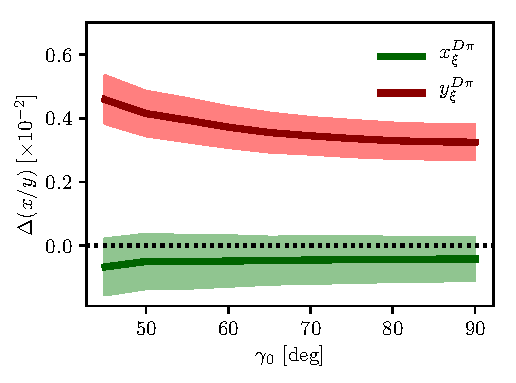
\includegraphics[width=0.45\columnwidth]{figures/ks_chapter/delta_xy_dpi.pdf}
  \caption{The bias on (left) the \BtoDK and (right) $\BtoDpi \;\CP$-violation observables in the \lhcb DD category, evaluated in bias studies with inputs based on full \lhcb simulation, calculated as a function of input $\gamma_0$.}
  \label{fig:LHCb_related_biases}
\end{figure}

As the statistical uncertainty becomes comparable with the bias effects described in this chapter, the systematic uncertainty should be assigned by a more accurate study, incorporating the traversed material on a track-by-track basis in full detector simulation. Such a detailed calculations can also be used to apply a bias correction if desired. 

% subsection the_impact_on_coupled_btodk_and_btodpi_measurements (end)

\section{Concluding remarks} % (fold)
\label{sec:concluding_remarks}

% subsection concluding_remarks (end)


The analysis presented in this chapter has shown the expected impact of neutral kaon \CP violation and material interaction on current BPGGSZ measurements to be small compared to the statistical uncertainties; first by simple order-of-magnitude estimates and then by a detailed calculation of the expected effect in \lhcb and Belle~II.



While the calculations were made for the case of \DtoKspipi decays, the BPGGSZ approach can of course also be applied in other \D-decay final states, such as ${\D\to\KS\Kp\Km}$ and $\D\to\KS\pip\pim\piz$. The biases on measurements of $\gamma$ based the \D decay phase-space distributions should be of similar size in these decay channels. The impact on $\gamma$ measurements based on the phase-space-integrated yield asymmetry can be expected to be tens of degrees for the $\D\to\KS\Kp\Km$ channel, where the yield asymmetry is expected to be around 2\,\%, for the reasons explained in Section~\ref{sub:modification_of_the_bpggsz_yield_equations}. The $\D\to\KS\pip\pim\piz$ decay, however, is dominantly \CP-odd~\cite{CLEOKSpipipi0}, and the bias in measurements based on the total asymmetry is therefore expected to be $O(\epsilon/r_B)$, ie. a few degrees~\cite{grossmanEffectsBarMixing2014}. More precise calculations of the biases would require a repeat of the study included here, with relevant amplitude models and binning schemes in place.



The chapter focuses on the model-independent, binned approach that is the subject of the thesis. However, the underlying mechanism that determines the scale of the bias, namely that the phase-space \emph{distribution} of signal decays is unaffected at $\mathcal O(\epsilon)$ and $\mathcal O(r_\chi)$, is independent on the exact measurement approach. Therefore it is expected that amplitude-model-based measurements and measurements made with new unbinned methods such as those in Ref~\cite{poluektovUnbinnedModelindependentMeasurements2018} will be similarly biased if kaon \CP violation and regeneration are not accounted for. 
% section impact_on_ggsz_measurements (end)

% section cp_violation_and_material_interaction_of_neutral_kaons (end)


